\documentclass[12pt,letterpaper]{article}

\usepackage{graphicx,amssymb,amsmath,bm,color,multicol}
\graphicspath{ {./images/} }
\usepackage{../newcommand}
\sloppy
\newcommand{\ignore}[1]{}

\newenvironment{proof}{\noindent{\bf Proof:}}{\qed\bigskip}

\newtheorem{theorem}{Theorem}
\newtheorem{corollary}{Corollary}
\newtheorem{lemma}{Lemma} 
\newtheorem{claim}{Claim}
\newtheorem{fact}{Fact}
\newtheorem{definition}{Definition}
\newtheorem{assumption}{Assumption}
\newtheorem{observation}{Observation}
\newtheorem{example}{Example}
\newcommand{\qed}{\rule{7pt}{7pt}}

\newcommand{\homework}[4]{
	\thispagestyle{plain} 
	\newpage
	\setcounter{page}{1}
	\noindent
	\begin{center}
		\framebox{ \vbox{ \hbox to 6.28in
				{\bf ECON 4190: Industrial Organization \hfill #1} %change course name
				\vspace{4mm}
				\hbox to 6.28in
				{\hspace{2.5in}\large\mbox{Homework #2}}
				\vspace{4mm}
				\hbox to 6.28in
				{{\it Collaborators: #3\hfill}}
			}}
		\end{center}
	}

\oddsidemargin 0in
\evensidemargin 0in
\textwidth 6.5in
\topmargin -0.5in
\textheight 9.0in

\begin{document}

% Modify this command to be your name and computing ID
\homework{Fall 2021}{$4$}{Alex Shen (as5gd), Sean Velhagen (spv5hq), Max Bresticker (mtb9sex)}

Pledge: On my honor, I pledge that I have neither given nor received help on this assignment 
Signature: \textit{Alex Shen, Sean Velhagen, Max Bresticker}

\begin{enumerate}
	
\item[1.] 
\begin{enumerate}
	\item As usual, we find $\hat{x}$, the indifferent consumer between Firms 1 and 2. Since $M=1$, this will also give us $Q_1$, the quantity produced by Firm 1, and therefore $1-\hat{x} = Q_2$, the quantity produced by Firm 2. Since the value for a consumer at $\hat{x}$ must be the same for both, assuming that the market is fully covered we can simply use the utility equation to solve for $\hat{x}$ as such:
	
	\begin{align*}
		R - p_1 - \tau \hat{x} &= R - p_2 - \tau(1-\hat{x}) \\
		p_2 - p_1 + 1 &= 2 \tau \hat{x} \\
		\hat{x} &= \frac{p_2 - p_1}{2\tau} + \frac{1}{2}
	\end{align*}

	Using $\hat{x}$ as $Q_1$, we maximize Firm 1's profit equation to solve for its reaction function for $p_1$, which will then give us Firm 2's reaction function for $p_2$ by symmetry:
	
	\begin{align*}
		max_{p_1} \pi_1 &= (\frac{p_2 - p_1}{2\tau} + \frac{1}{2})(p_1 - c_1) \\
		\frac{\partial \pi}{\partial p_1} &= (-\frac{1}{2\tau})(p_1 - c) + \frac{p_2 - p_1}{2\tau} + \frac{1}{2} = 0 \\
		0 &= \frac{p_2 - p_1 - (p_1 - c_1)}{2\tau} + \frac{1}{2} \\
		&= \frac{p_2 - 2p_1 + c}{2\tau} + \frac{1}{2} \\
		\therefore p_1^* &= \frac{p_2 + c_1 + \tau}{2} \\ 
		\therefore p_2^* &= \frac{p_1 + c_2 + \tau}{2}
	\end{align*}

	Plugging Firm 2's reaction function into Firm 1's allows us to solve for $p_1^*$ and then $p_2^*$:

	\begin{align*}
		p_1 &= \frac{\frac{p_1 + c_2 + \tau}{2} + c_1 + \tau}{2} \\
		4p_1 &= p_1 + c_2 + \tau + 2c_1 + 2\tau \\
		p_1^* &= \tau + \frac{2c_1 + c_2}{3} \\ 
		\therefore p_2^* &= \tau + \frac{2c_2 + c_1}{3}
	\end{align*}

	{\color{blue}\textbf{Solution:} In Bertrand-Nash equilibrium, $p_1^* = \tau + \frac{2c_1 + c_2}{3}$, $p_2^* = \tau + \frac{2c_2 + c_1}{3}$}

	\item When colluding, the firms will set prices such that the indifferent consumer receives a utility of 0, which minimizes total consumer surplus (thus maximizing producer surplus/profit). Plugging back the calculated $\hat{x}$ into our value functions gives us the following:
	
	\begin{multicols}{2}
		\noindent
		\begin{align*}
			R - p_1 - \tau (\frac{p_2 - p_1}{2\tau} + \frac{1}{2}) = 0
		\end{align*}
		\noindent
		\begin{align*}
			&R - p_2 - \tau (1 - ((\frac{p_2 - p_1}{2\tau} + \frac{1}{2}))) = 0 \\
			&R - p_2 - \tau (\frac{p_1 - p_2}{2\tau} + \frac{1}{2}) = 0
		\end{align*}
	\end{multicols}

	Given the symmetry we see in these equations, we can conclude that $p_1 = p_2$. This also makes sense intuitively both because this sets the indifferent consumer point exactly between them, and means they split the profit evenly. In any case, redoing our equation with $p_1 = p_2$ gives us $p_1 = R - \frac{\tau}{2} = p_2$.

	{\color{blue}\textbf{Solution:} If colluding, Firms 1 and 2 will both set their price to $R - \frac{\tau}{2}$.}

	\item To verify sustainability, we simply assume that a given firm (say, Firm 2) is using that price, use the reaction function for the other firm (Firm 1 in this case) to see what its best response is, and see if the value matches the collusion price.
	
	\begin{align*}
		p_1^*(p_2) &= \frac{p_2 + c_1 + \tau}{2} \\
		p_1^*(R - \frac{\tau}{2}) &= \frac{R - \frac{\tau}{2} + c_1 + \tau}{2} \\
		&= \frac{R + c_1}{2} + \frac{\tau}{4}
	\end{align*}

	This is obviously not the same thing as the collusion price, so Firm 1 will deviate from colluding. Because of symmetry, we also know that Firm 2 will deviate for similar reasons. Thus, collusion is not sustainable.

	{\color{blue} \textbf{Solution:} No, collusion is not sustainable.}
\end{enumerate} 

\item[2.]

\begin{enumerate}
	\item Given $Q = 200 - 2P$, we know that $P = 100 - \frac{1}{2}Q$. If Apple is a monopolist with $MC = 4$, its profit can be determined by $\pi(Q) = (P-C)Q =  (100 - \frac{1}{2}Q - 4) (Q)$. Thus, the first order condition for this equation is $\frac{d \pi}{d P} = 96 - Q = 0$, meaning that $Q^M = 96$. Plugging this value back into our previous equations gives us $P^M = 52$ and $\pi^M = 96 * (52- 4) = 4608$.
	
	{\color{blue}\textbf{Solution:} $Q^M = 96$, $P^M = 52$, $\pi^M = 4608$}

	\item Since a competitive firm supplies along its MC curve (meaning that $p = MC$, which we know to be true in perfect competition), to solve for a given firm's quantity produced, $q$, we simply substitute in price and invert their MC function to get $q = \frac{p-20}{6}$. Since there are 12 identical firms in the fringe, the fringe supply is in total $12 * (\frac{p-20}{6}) = 2p - 40$. Importantly, we have to also add the constraint that this curve only holds when $p \geq 20$, as otherwise the firm would be producing a negative quantity which is impossible.
	
	{\color{blue}\textbf{Solution:} $Q_{fringe} = 2p - 40$ if $p \geq 20$, otherwise 0}

	\item We first find the residual demand for Apple's product ($Q_{Apple}$) by subtracting the quantity the fringe will produce ($Q_{fringe}$) at a given price from the total market demand ($Q_{market}$) at a given price.
	\begin{align*}
		Q_{Apple} &= Q_{market} - Q_{fringe} \\
		&= 200 - 2P - (2P - 40) \\
		&= 240 - 4P \\
		\therefore P &= 60 - \frac{1}{4}Q_{Apple}
	\end{align*}

	We then maximize the resulting profit function to determine $Q_{Apple}$:

	\begin{align*}
		max_{Q_{Apple}} \pi &= (60 - \frac{1}{4}Q_{Apple} - 4) * Q_{Apple} \\
		\frac{d\pi}{d Q_{Apple}} &= 56 - \frac{1}{2} Q_{Apple} = 0 \\
		\therefore Q_{Apple} &= 56 * 2 = 112
	\end{align*}

	From there, everything else is straightforward - plug in $Q_{Apple}$ to find $P = 60 - \frac{112}{4} = 32$, which then gives us $Q_{fringe} = 2(32) - 40 = 24$ and $\pi_{Apple} = (56 - \frac{112}{4}) * 112 = 3136$.

	{\color{blue}\textbf{Solution:} $Q_{Apple} = 112$, $P = 32$,  $Q_{fringe} = 24$,  $\pi_{Apple} = 3136$}

	\item Graph as shown:
	
	{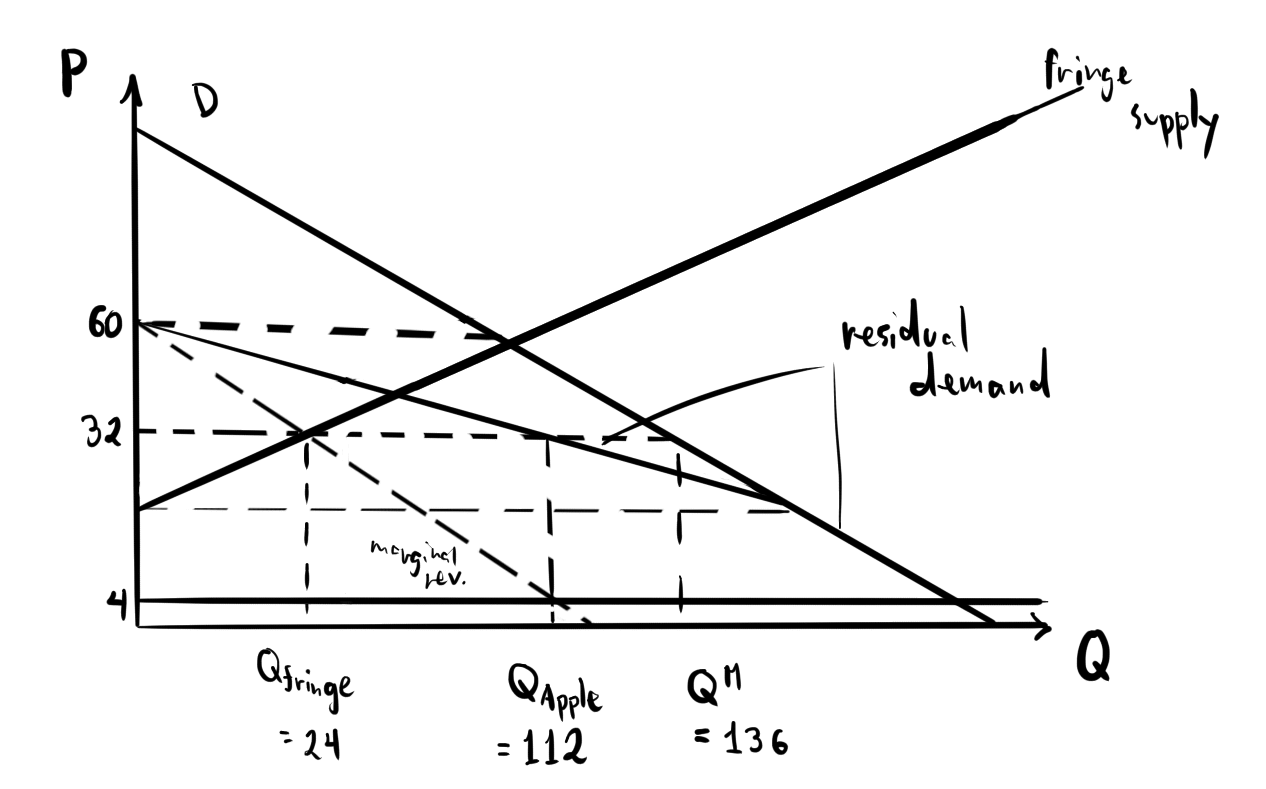
\includegraphics[width=\textwidth]{2d.png}}
\end{enumerate}

\item[3.] From $TC(Q) = 8Q$, we know that $MC = 8$. Total quantity demanded by the market is $Q = 56 - P$, so subtracting $Q_{fringe}$ to find Britney's residual demand gives us $Q_{B} = 56 - P - (2P - y) = 56 - 3P + y$. We then maximize her derived profit function as follows to find the relationship between $y$ and $P^*$:

\begin{align*}
	max_{p} \pi_B &= (56 - 3P + y) * (p - 8) \\
	FOC: \frac{d \pi}{d p} &= (56 - 3P + y) - (-3)(p - 8) = 0\\
	0 &= 56 - 3P + y - 3P + 24 \\
	0 &= 80 - 6P + y \\
	y &= 6P - 80
\end{align*}

Since we know that $P=16$, simple substitution yields that $y = 6 * 16 - 80 = 16$, which gives us $Q_B = 56 - 3*16 + 16 = 24$ and $Q_{fringe} = 2*16 - 16 = 16$.

{\color{blue}\textbf{Solution:} $y = 16$, $Q_B = 24$, $Q_{fringe} = 16$ }

\end{enumerate}
	
\end{document}
